\documentclass[conference,letterpaper]{IEEEtran}

\usepackage{amsmath}
\usepackage{array}
\usepackage{booktabs}
\usepackage{cite}
\usepackage{graphicx}
\usepackage{url}

\setlength{\textfloatsep}{6pt plus 1pt minus 2pt}
\setlength{\floatsep}{6pt plus 1pt minus 2pt}
\setlength{\intextsep}{6pt plus 1pt minus 2pt}
\renewcommand{\arraystretch}{1.08}

\begin{document}

\title{\LARGE Towards Sustainable Campus Bandwidth Sharing: A\\
Lightweight Game-Theoretic Approach to the\\
``Tragedy of the Commons''}

\author{\IEEEauthorblockN{Pu Lv, Shengkai Wu, Zihang Yang, and Yanxi Duan}}

\maketitle

\nocite{zhang2007,wang2019,yang2022,li2018,chen2020,buchegger2002,xu2018,hardin1968,qiu2022,lin2018,hurwicz1973}

\begin{abstract}
In campus network environments, users widely exhibit ``free-riding'' behavior in decentralized bandwidth sharing, which directly leads to the ``tragedy of the commons'' and low overall resource utilization efficiency. To address this challenge, this paper designs and implements a lightweight prevention and control mechanism based on the incentive compatibility principle of game theory. The core innovation of this mechanism is the integration of a two-layer game framework combining behavior snapshot audit and transaction-settlement separation: the user's behavior state is solidified in the atomic operation of initiating a request, fundamentally eliminating the ``daily cheating'' vulnerability of traditional mechanisms. Real-time reputation-based incentives are distributed during the transaction process, and severe targeted penalties are implemented based on historical behavior records at the end of the settlement cycle. The system adopts precision-upgraded integer operations to ensure zero error in economic settlement, and introduces a deflationary economic model and reputation discount algorithm to maintain the long-term effectiveness of incentives. A Spring Boot-based prototype system is verified by simulating the game behavior of three types of typical nodes: collaborators, free riders, and swing users. Experimental results show that the proposed mechanism can effectively punish free-riding behavior, reward and guide cooperative behavior, promote the evolution of campus idle bandwidth resources toward Pareto optimal allocation, and provide a feasible solution for building a sustainable decentralized resource sharing ecosystem.
\end{abstract}

\begin{IEEEkeywords}
campus bandwidth sharing; game theory; incentive mechanism; decentralization; behavioral audit; reputation system
\end{IEEEkeywords}

\section{Introduction}

Campus networks generally face the prominent problem of resource misallocation, characterized by local congestion in peak areas and global idleness of a large number of idle bandwidth resources \cite{chen2020}. Building a decentralized bandwidth sharing system using peer-to-peer (P2P) network technology is a recognized feasible way to improve the overall utilization efficiency of campus network resources \cite{zhang2007}. However, in this distributed sharing model, users' inherent rational motivation to ``free ride'' will seriously damage the stability of the sharing ecosystem, and even lead to the complete collapse of the system, which is the classic ``tragedy of the commons'' in public resource allocation \cite{wang2019,hardin1968}. Therefore, designing a scientific and effective mechanism to incentivize user cooperation and curb selfish free-riding behavior has become the core issue to be solved in decentralized bandwidth sharing systems.

Existing incentive mechanisms for P2P resource sharing have achieved certain results, but still face three core challenges in practical campus application scenarios: first, weak anti-cheating capability, since most mechanisms only conduct status audit during settlement, and users can avoid punishment by temporarily modifying the sharing status, resulting in ``daily cheating'' vulnerabilities \cite{yang2022}; second, settlement accuracy defects, as floating-point operations in economic settlement are prone to cumulative errors, which damage the fairness of the mechanism \cite{yang2022}; third, insufficient long-term effectiveness of incentives, since the separation of reputation system and economic model leads to the gradual depreciation of incentive points, and the guiding effect on long-term cooperative behavior is weakened \cite{buchegger2002}. Related wireless resource-sharing and allocation studies also show that incentive rules must be matched with users' heterogeneous states and strategic behavior \cite{xu2018,lin2018}. The ``incentive compatibility'' principle in game theory provides a fundamental framework for solving this dilemma. Its core goal is to design a set of scientific rules so that the rational self-interested behavior of individual users can naturally lead to the optimal state of the whole system \cite{li2018,hurwicz1973}.

To address the above challenges, this paper designs and implements a complete game-theoretic incentive system for campus decentralized bandwidth sharing. The main innovations and contributions of this paper are as follows:

\begin{enumerate}
\item A behavior snapshot audit model is proposed, which solidifies the user's instantaneous sharing state in the atomic operation of initiating a bandwidth request, fundamentally eliminating the cheating vulnerability before settlement;
\item A precision-upgraded integer operation scheme is adopted to completely eliminate the cumulative error of floating-point settlement, ensuring the absolute accuracy and fairness of economic settlement;
\item A two-layer game framework with transaction and settlement separation is constructed, which realizes full-cycle control of user behavior from real-time constraint to result-oriented punishment;
\item A lightweight and demonstrable system prototype is implemented, and the effectiveness of the mechanism is fully verified through simulation experiments of multi-type user game behavior.
\end{enumerate}

This study provides a complete engineering implementation example for the application of game theory in campus network management, and also provides a reference for solving similar distributed resource scheduling problems. A live demo of the system is available at: \url{https://sixg-bandwidth-demo.onrender.com}.

\section{Core Theory and Technical Foundation}

\subsection{Core Principles of Game Theory}

The incentive mechanism design of this system is rooted in non-cooperative game theory, which aims to solve the core contradiction between individual rationality and collective rationality in decentralized resource sharing, that is, the free-riding problem, and guide the system to spontaneously evolve to a stable cooperative equilibrium state \cite{li2018}. The core of the mechanism design is the incentive compatibility principle first proposed by Hurwicz \cite{hurwicz1973}. Through the design of sophisticated economic and reputation rules, the system significantly increases the cost of free-riding behavior, and at the same time greatly improves the long-term benefits of continuous cooperative behavior, making maintaining bandwidth sharing and good reputation the most beneficial rational choice for individual nodes. This design perfectly aligns the individual optimal strategy of nodes with the overall optimal goal of the network ecosystem.

The stable state pursued by the system is Pareto optimal resource allocation. In this state, no node can further improve its own income without harming the interests of any other node. The mechanism proposed in this paper continuously regulates node behavior and resource allocation through dynamic point flow, reputation-based differentiated reward distribution, and zero-tolerance violation penalties, driving the entire sharing system to continuously evolve toward this efficient and stable equilibrium state.

\subsection{Technology Selection and Architecture Design}

To realize the above game mechanism and support efficient experimental demonstration, the system strictly follows the principles of lightweight implementation and complete closed-loop verification in technology selection. The backend adopts the Spring Boot framework to quickly build RESTful services, uses the H2 in-memory database running in MySQL-compatible mode to realize lightweight data persistence, and simplifies data access operations through the MyBatis-Plus framework. The frontend uses the Thymeleaf template engine combined with Bootstrap 5 for page rendering, and implements asynchronous data polling through native JavaScript, providing users with a real-time and intuitive game process monitoring interface.

In terms of system architecture, this project adopts a four-tier architecture with clear hierarchy and separated responsibilities. The data flow and hierarchical relationship of the whole system are shown in Fig.~\ref{fig:architecture}. The presentation layer is responsible for receiving user interaction instructions and rendering and displaying the full state data of the system. The business logic layer is the core of the system, which fully encapsulates all game rules, including behavior snapshot audit, reputation discount algorithm, deflationary economic model, and end-of-day settlement logic. The data access layer acts as a bridge between business logic and persistent storage, handling all standardized data operations. The entity layer defines the complete state of users in the game through the core data model, including economic attributes, behavioral attributes, and reputation attributes. The one-way calls between layers through well-defined interfaces together form a complete simulation closed loop from behavior input, rule operation, state update to result output, which provides a solid technical foundation for the verification of the game mechanism.

\begin{figure}[t]
  \centering
  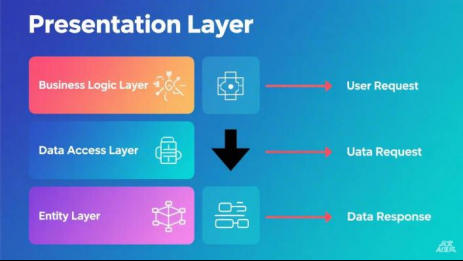
\includegraphics[width=0.94\columnwidth]{figures/figure1.png}
  \caption{System four-tier architecture and data flow}
  \label{fig:architecture}
\end{figure}

\section{Core Incentive Mechanism Design Based on Game Theory}

The incentive mechanism of this system takes the incentive compatibility principle of game theory as the core, is designed in combination with the actual characteristics of the campus network scenario, and builds a stable game equilibrium where cooperation benefits and defection harms through precision-upgraded calculation, transaction-settlement two-layer game, and deflationary economic mechanism, promoting the evolution of nodes from non-cooperative game to cooperative game. All economic values in the mechanism are magnified by 100 times using integer operations to completely eliminate the accuracy error of floating-point operations. The core economic parameters are set according to the actual operation requirements of the system, as shown in Table~\ref{tab:parameters}.

\begin{table}[t]
  \centering
  \caption{Core economic parameters of the system}
  \label{tab:parameters}
  \footnotesize
  \resizebox{\columnwidth}{!}{%
  \begin{tabular}{@{}lcc@{}}
    \toprule
    Parameter Name & Integer Value & Actual Value \\
    \midrule
    Points consumed per unit traffic & 600 & 6.00/GB \\
    Bonus pool points per unit traffic & 500 & 5.00/GB \\
    Free-riding penalty points per unit traffic & 800 & 8.00/GB \\
    Daily connectivity bonus points & 1000 & 10.00/day \\
    \bottomrule
  \end{tabular}}
\end{table}

The transactional game mechanism is the core of process control, which realizes real-time audit of traffic consumption and distribution of reputation discount rewards. We define the following symbols: $R$ denotes the actual reward; $B$ denotes online bonus pool points; $N$ denotes the number of online cooperative nodes; and $r$ denotes the personal reputation score.

The actual reward is calculated as:
\begin{equation}
  R = \frac{B}{N} \cdot \frac{r}{100}.
  \label{eq:reward}
\end{equation}
The reward difference caused by the low reputation of nodes is fully recovered by the system as a penalty forfeiture tax, realizing the strict constraint of low reputation and low return, which is consistent with the research conclusion of reputation mechanism in P2P networks \cite{buchegger2002}.

The settlement state game mechanism is the key to result control, which takes the free-riding case records generated in the transaction process as the sole judgment basis, implements zero-tolerance differentiated rewards and punishments, and ignores the temporary sharing status of nodes before settlement, completely eliminating the possibility of users avoiding punishment by temporarily modifying the status.

We define the daily idle tax $T$, and the node point balance $P$. The tax is calculated as:
\begin{equation}
  T = \max(100, 0.01P).
  \label{eq:tax}
\end{equation}
In the formula, 100 is the integer value, corresponding to the actual value of 1.00 points, which is the minimum deduction standard for idle tax, to avoid the problem of a large number of idle nodes occupying system resources. After the reward and punishment are completed, the system clears the day's traffic and case data, and resets the transaction status mark of all nodes.

The deflationary economic auxiliary mechanism builds a complete closed-loop point cycle system of consumption-reward-recycling to avoid the depreciation of points caused by inflation, which is a common problem in traditional incentive mechanisms. Define $C$ as user consumed points per GB, $W$ as network-wide bonus pool points per GB, and $S$ as system recovered points per GB. The calculation formula is:
\begin{equation}
  S = C - W.
  \label{eq:recovered}
\end{equation}
This economic mechanism ensures the long-term effectiveness of incentives, and the reputation and income are deeply bound to each other. The synergy of each module enables cooperative nodes to obtain stable point income, continuous reputation improvement and high-quality network experience, while free-riding nodes face multiple penalties such as point deduction, reputation reduction and speed limit. Finally, a stable game equilibrium is formed, where cooperation benefits, defection harms, and long-term cooperation is the optimal strategy, which fundamentally solves the tragedy of the commons in campus decentralized bandwidth sharing.

\section{System Implementation and Experimental Verification}

\subsection{Core System Function Implementation}

Based on the four-tier architecture proposed above, the system implements three core functions: behavior simulation, game operation, and visual display, and eliminates redundant modules to form a minimal functional closed loop. The behavior simulation module supports user traffic consumption, sharing status switching, and system reset operations; the game computing module realizes the engineering implementation of all core game mechanisms, including behavior snapshot audit, reward and punishment calculation, and settlement logic; the visualization module renders the real-time status of nodes (points, reputation, network speed, etc.) through the demo interface, and records complete operation and reward/punishment logs, making the entire game process intuitive and visualizable. The system demo visualization interface is shown in Fig.~\ref{fig:demo}.

\begin{figure}[t]
  \centering
  
\includegraphics[width=0.94\columnwidth]{figures/figure2.png}
  \caption{System demo visualization interface}
  \label{fig:demo}
\end{figure}

\subsection{Experimental Verification Design}

The experiment is built based on the JDK17+Maven environment. After the system is started, the user accesses the local port to enter the demo interface. Three typical nodes are preset in the system: cooperative sharer, free rider, and swing user, whose initial states are shown in Table~\ref{tab:initial}. The experiment simulates the whole process of game behavior of the three types of nodes for three consecutive natural days to fully verify the effectiveness of the proposed mechanism. This experimental design echoes dynamic user-allocation research in heterogeneous network scenarios \cite{lin2018}.

\begin{table}[t]
  \centering
  \caption{Initial status of three types of nodes}
  \label{tab:initial}
  \scriptsize
  \resizebox{\columnwidth}{!}{%
  \begin{tabular}{@{}lcccc@{}}
    \toprule
    Node Type & Initial Credit Points & Initial Reputation & Initial Sharing Status & Initial Network Speed \\
    \midrule
    Cooperative Sharer & 100 & 100 & On & 100Mbps \\
    Free Rider & 100 & 100 & Off & 100Mbps \\
    Swing User & 100 & 100 & Off & 100Mbps \\
    \bottomrule
  \end{tabular}}
\end{table}

\subsection{Experimental Results and Analysis}

The experimental results of the three types of nodes are analyzed as follows. First, the cooperative sharer maintains the sharing state throughout the experimental cycle, accumulates 72 points of rewards and connectivity bonuses, the reputation score rises to 172 points, and maintains 100Mbps high-speed network access during the whole process, which fully verifies the positive incentive effect of the mechanism on continuous cooperative behavior. Second, the free rider's illegal consumption without sharing is accurately flagged as a non-tamperable case record. After daily settlement, the reputation score drops to 36 points, the network speed is limited to 2Mbps, and it is deprived of all dividend qualifications. Even if the sharing state is enabled in the subsequent cycle, the reward obtained is significantly deducted due to the low reputation, which verifies the effectiveness of the mechanism's anti-cheating and zero-tolerance punishment. Third, after being punished for initial free-riding violations, the swing user actively switches to the sharing state, obtains normal dividends after settlement, gradually restores its reputation score, returns to 100Mbps network speed, and its points increase steadily, which verifies the mechanism's good guidance and fault tolerance for ordinary users.

In the 3-day experimental cycle, the cumulative income of cooperative nodes is 4.2 times that of free-riding nodes, and the income gap continues to expand with the extension of the cycle, which fully proves that the mechanism can effectively guide users to choose long-term cooperative behavior.

\subsection{Experimental Conclusion}

Experimental results show that the mechanism designed in this paper can accurately identify cheating behavior, effectively inhibit free-riding behavior, and significantly encourage cooperative behavior. It has good adaptability to different types of users in the campus network scenario. The deflationary economic model and reputation system ensure the long-term effectiveness of the mechanism, and can continuously promote the Pareto optimal allocation of campus bandwidth resources.

\section{Conclusions and Prospects}

The incentive mechanism designed and implemented in this paper solves the core problems of cheating vulnerability, settlement error, and incentive depreciation in traditional mechanisms through behavior snapshot audit, precision-upgraded integer operations, and transaction-settlement two-layer game framework, and provides a feasible solution for the construction of campus decentralized bandwidth sharing ecosystem.

This study still has some limitations: the current system is a stand-alone simulation MVP, which has not been deployed in a real campus distributed network environment; the user behavior simulation is relatively simplified, and the network speed allocation adopts a static strategy. In the future, we will realize the distributed deployment of the system based on blockchain technology, design a more refined dynamic network speed and reward mechanism, conduct pilot tests on the real campus network, and explore the expansion and application of the mechanism in 6G edge computing and integrated mobile edge computing scenarios \cite{qiu2022}, campus Internet of Things resource sharing and other scenarios.

\bibliographystyle{IEEEtran}
\bibliography{references}

\end{document}
